Due to some technical issues, we had to reset our EC2 instance, thus the findings presented are those collected following the reset. As of the writing of this paper, we have made over 20,000 detections on our honeypots. Modern Honeypot Network provides some useful high level statistics about our honeypots some of which may be seen in Table 1 and Table 2. Another interesting observation is that the vast majority of our data came from Snort, as over 13,500 detections originated from our Snort honeypot.

We also found that 1433 was attacked significantly than any other port for a given 24 hour period. This is likely due to port 1433's use as the default port for many SQL servers.


\begin{table}[H]
	\resizebox{\columnwidth}{!}{%
	\begin{tabular}{|c|c|c|}
		\hline
		IP Address (first 5 digits) & Country     & Number of attacks (last 24 hours) \\ \hline
		83.97.2                 & Romania     & 19                \\ \hline
		89.248                & Netherlands & 18                \\ \hline
		185.15                & Russia     & 18                \\ \hline
		77.247                 & Netherlands & 17                \\ \hline
		185.15                & Russia      & 16                \\ \hline
	\end{tabular}%
	}
\caption{Top Five Individual Detected IP Addresses} \label{tab:ips}
\end{table}

\begin{table}[H]
	\resizebox{\columnwidth}{!}{%
	\begin{tabular}{|c|c|c|}
		\hline
		Attacked Port & Number of Attacks & Common Port Use                                                                               \\ \hline
		1433          & 182               & SQL Server                                                                                    \\ \hline
		5060          & 87                & Clear Text SIP, VoIP                                                                          \\ \hline
		22            & 53                & SSH                                                                                           \\ \hline
		8545          & 17                & Remote Procedure Call interface of Ethereum clients \\ \hline	
		443           & 16                & https                      \\ \hline
	\end{tabular}%
	}
\caption{Top Five Attacked Ports} \label{tab:ports}
\end{table}

Using the \href{https://github.com/pieqq/PyGeoIpMap}{PyGeoIpMap} library, we were also able to plot the approximate locations of attacker IP addresses (Figure 1). Additionally, we plotted the top 20 countries by attacker, as seen in Figure 2. While IP addresses from all around the world were detected, the majority came from the United States, the Netherlands, China, Russia, and Germany. One note of importance regarding IP addresses is that the addresses we've encountered are not necessarily those of the attacker since attackers could be using VPNs.

\begin{figure}[H]
	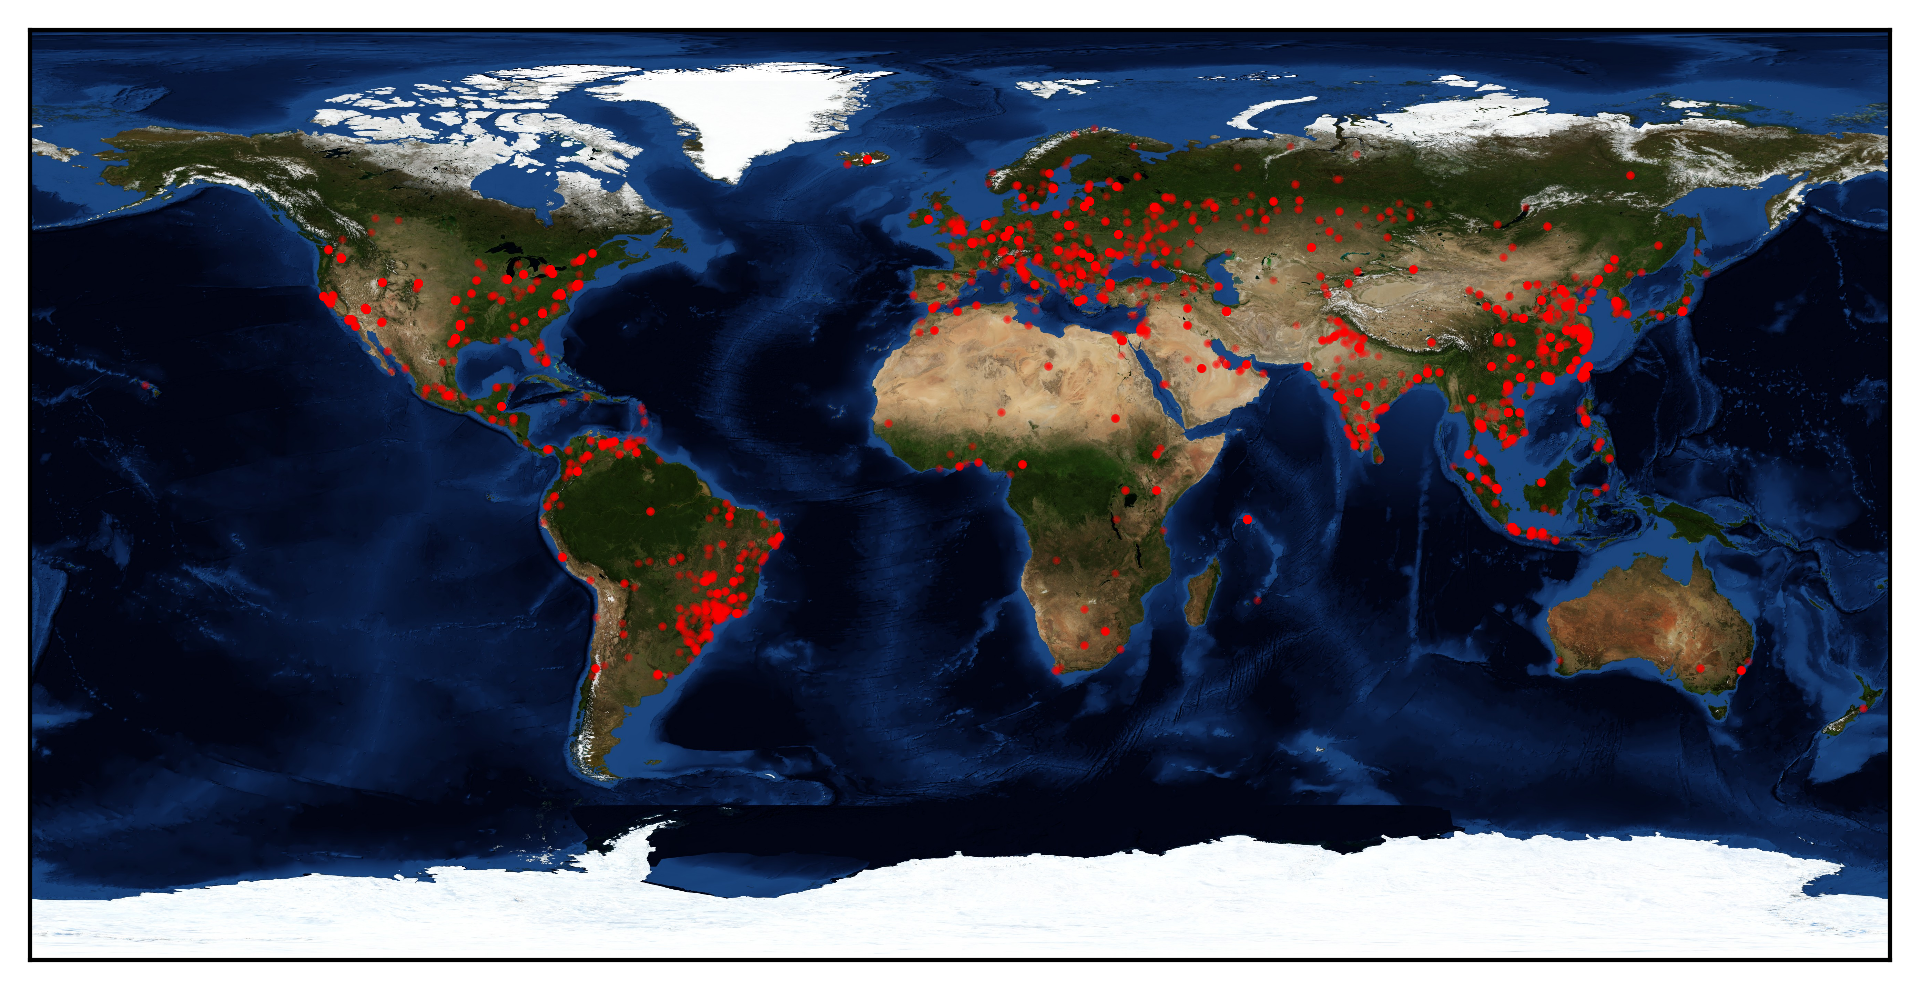
\includegraphics[width=\linewidth]{map.png}
	\caption{Approximate Locations of Attacker IP Addresses.}
	\label{fig:map}
\end{figure}


\begin{figure}[H]
	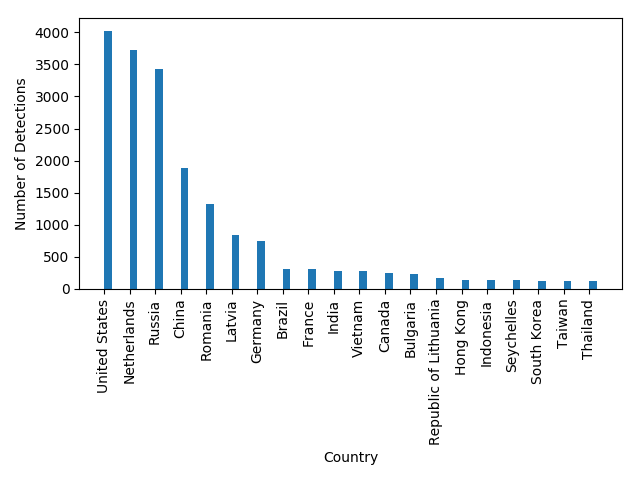
\includegraphics[width=\linewidth]{top_countries.png}
	\caption{Top Detected Countries.}
	\label{fig:top-countries}
\end{figure}

We also explored the types of operating systems detected. Most operating systems were either Linux 2.2-3.x of some barebones variety or Windows 7/8. Unfortunately for most detections we were not actually able to determine the operating system. The breakdown of detected operating systems can be seen in Figure 3.

\begin{figure}[H]
	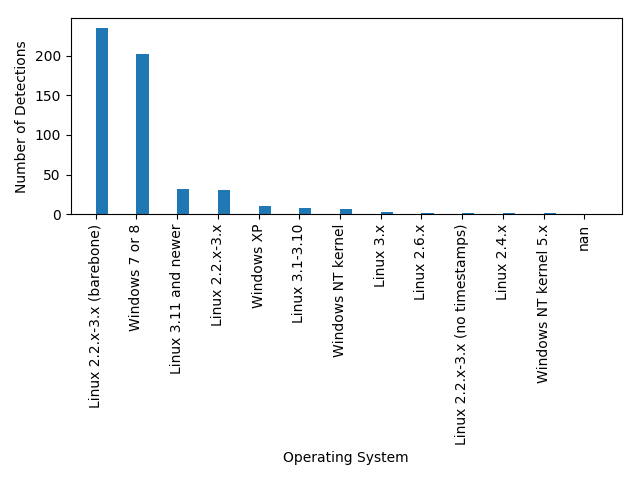
\includegraphics[width=\linewidth]{top_os.png}
	\caption{Top Detected Operating Systems.}
	\label{fig:top-os}
\end{figure}

The final datapoint we explored was the time of detection. The full breakdown of attacks can be seen in Figure 4. From our findings we can see that, for the most part, most detections cam during the first half of the day (relative to UTC). However, there nearly always seemed to be some detections occurring. 

\begin{figure}[H]
		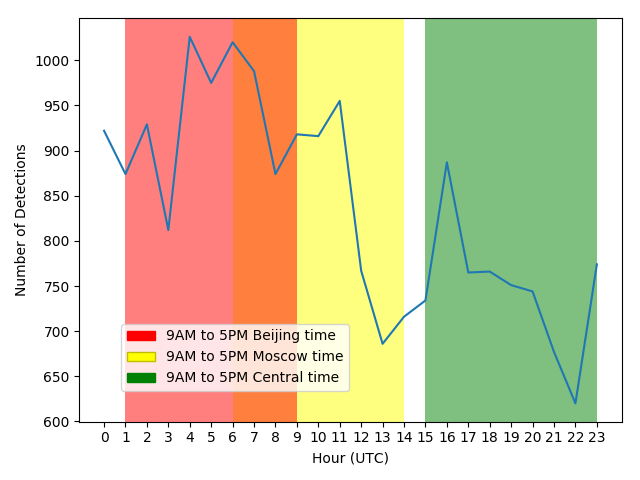
\includegraphics[width=\linewidth]{time_breakdown.png}
	\caption{Detections by Time}
	\label{fig:top-time}
\end{figure}

While we were able to detect a great deal of information, it is difficult to determine the exact intent of all those we detected. In some cases, we can see that SSHing  and crypto mining were attempted. In other cases, we can only see that an https request was made. That being the case, the line is blurred when attempting to divide detections into malicious and non-malicious activity.